\documentclass[tikz,border=8pt]{standalone}
\usepackage{amsmath}
\usepackage{amssymb}
\usetikzlibrary{arrows.meta,calc,decorations.pathreplacing,patterns,shapes.geometric,positioning,shadings,3d}

\begin{document}
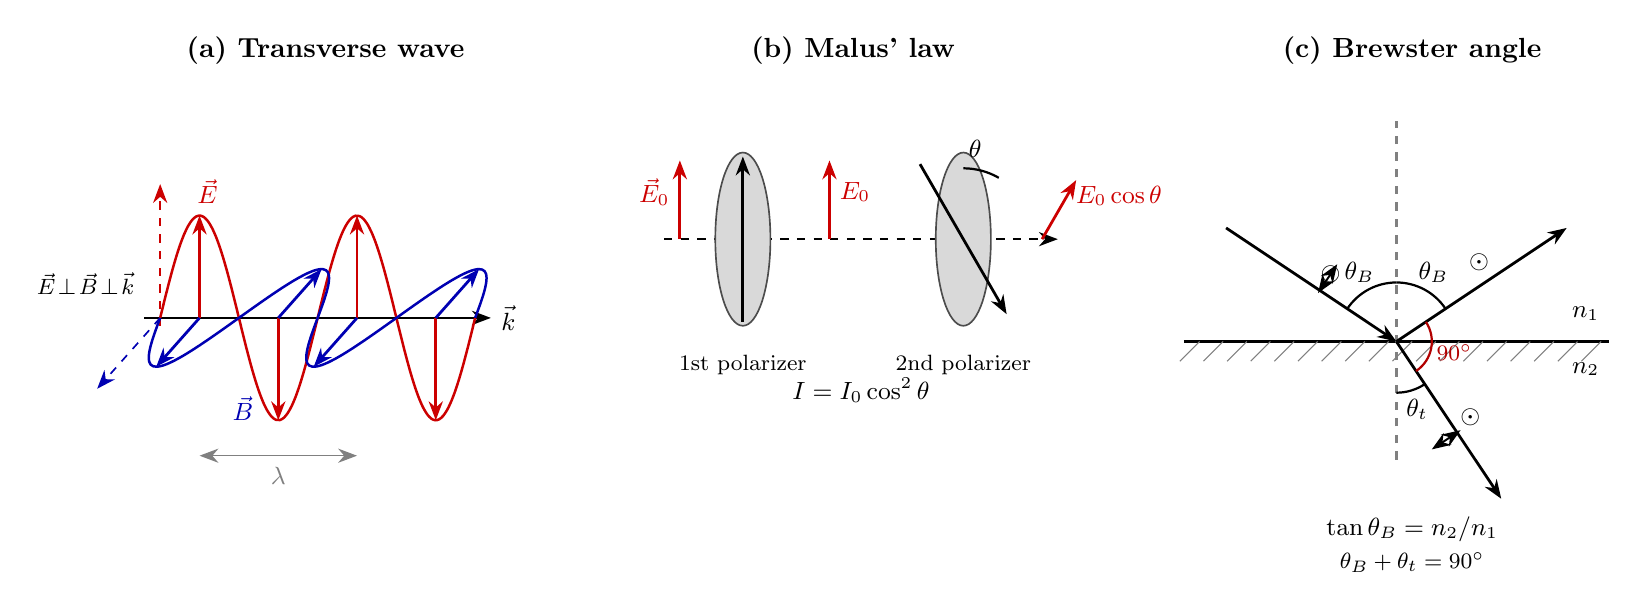
\begin{tikzpicture}[>={Stealth[length=2.4mm,width=1.8mm]},line width=0.8pt,font=\small]

% =====================================================
% (a) 3D electromagnetic wave: E, B, k orthogonal triad
% =====================================================
\begin{scope}[xshift=0cm]
  \node[font=\bfseries,anchor=north] at (2.1,3.7) {(a) Transverse wave};

  % axes (perspective): k along right, E up, B into page-ish
  % We'll use a simple isometric-ish projection
  % k axis (propagation, black)
  \draw[->,black,line width=1pt] (-0.2,0) -- (4.2,0) node[right]{$\vec{k}$};
  % E axis up (red) reference
  \draw[->,red!80!black,line width=0.6pt,dashed] (0,-0.1) -- (0,1.7);
  % B axis (blue) into perspective direction
  \draw[->,blue!70!black,line width=0.6pt,dashed] (0,0) -- (-0.8,-0.9);

  % sinusoidal E field (red, vertical) along k
  \draw[red!80!black,line width=0.9pt,smooth,samples=80,domain=0:4]
    plot (\x, {1.3*sin(\x*180)});
  % E vectors at peaks
  \foreach \x in {0.5,1.5,2.5,3.5}{
    \draw[->,red!80!black,line width=1pt] (\x,0) -- (\x,{1.3*sin(\x*180)});
  }

  % sinusoidal B field (blue, into-page direction) along k
  \draw[blue!70!black,line width=0.9pt,smooth,samples=80,domain=0:4]
    plot ({\x - 0.55*sin(\x*180)}, {-0.62*sin(\x*180)});
  \foreach \x in {0.5,1.5,2.5,3.5}{
    \draw[->,blue!70!black,line width=1pt] (\x,0) -- ({\x - 0.55*sin(\x*180)}, {-0.62*sin(\x*180)});
  }

  % Labels on the wave
  \node[red!80!black] at (0.6,1.6) {$\vec{E}$};
  \node[blue!70!black] at (1.05,-1.15) {$\vec{B}$};

  % wavelength indication
  \draw[<->,gray,line width=0.5pt] (0.5,-1.75) -- (2.5,-1.75);
  \node[gray] at (1.5,-2.0) {$\lambda$};

  % Small triad at origin
  \node[anchor=north east,font=\footnotesize] at (-0.2,0.7) {$\vec{E}\!\perp\!\vec{B}\!\perp\!\vec{k}$};
\end{scope}


% =====================================================
% (b) Malus law: two polarizers
% =====================================================
\begin{scope}[xshift=6.8cm]
  \node[font=\bfseries,anchor=north] at (2.0,3.7) {(b) Malus' law};

  % beam axis
  \draw[->,black,line width=0.7pt,dashed] (-0.4,1.0) -- (4.6,1.0);

  % First polarizer (gray disk) - front
  \draw[fill=gray!30,draw=gray!60!black,line width=0.6pt] (0.6,1.0) ellipse (0.35 and 1.1);
  \node[below=4pt] at (0.6,-0.2) {\footnotesize 1st polarizer};
  % transmission axis on first polarizer (vertical)
  \draw[->,black,line width=1pt] (0.6,-0.05) -- (0.6,2.05);

  % Second polarizer (gray disk)
  \draw[fill=gray!30,draw=gray!60!black,line width=0.6pt] (3.4,1.0) ellipse (0.35 and 1.1);
  \node[below=4pt] at (3.4,-0.2) {\footnotesize 2nd polarizer};
  % transmission axis tilted by theta=30deg from vertical
  \draw[->,black,line width=1pt] ($(3.4,1.0)+(120:1.1)$) -- ($(3.4,1.0)+(-60:1.1)$);

  % Incoming E0 vector (red) before first polarizer
  \draw[->,red!80!black,line width=1pt] (-0.2,1.0) -- (-0.2,2.0);
  \node[red!80!black,left] at (-0.2,1.6) {$\vec{E}_0$};

  % E0 after first polarizer (red, vertical)
  \draw[->,red!80!black,line width=1pt] (1.7,1.0) -- (1.7,2.0);
  \node[red!80!black,right] at (1.7,1.6) {$E_0$};

  % After second polarizer: projection E0 cos theta along tilted axis
  % tilted axis direction: 60 deg from horizontal (i.e., theta=30 from vertical)
  \draw[->,red!80!black,line width=1pt] (4.4,1.0) -- ($(4.4,1.0)+(60:{1.0*cos(30)})$);
  \node[red!80!black,right] at (4.7,1.55) {$E_0\cos\theta$};

  % angle arc between first (vertical) and second (tilted) axes near 2nd polarizer
  \draw[thick] (3.4,1.9) arc[start angle=90,end angle=60,radius=0.9];
  \node at (3.55,2.15) {$\theta$};

  % formula
  \node[anchor=south,font=\small] at (2.1,-1.2) {$I=I_0\cos^2\theta$};
\end{scope}


% =====================================================
% (c) Brewster angle geometry
% =====================================================
\begin{scope}[xshift=13.6cm,yshift=-0.3cm]
  \node[font=\bfseries,anchor=north] at (2.3,4.0) {(c) Brewster angle};

  % interface horizontal line
  \draw[black,line width=0.9pt] (-0.6,0) -- (4.8,0);
  % hatching below (denser medium n2)
  \foreach \x in {-0.4,-0.1,0.2,0.5,0.8,1.1,1.4,1.7,2.0,2.3,2.6,2.9,3.2,3.5,3.8,4.1,4.4,4.7}{
    \draw[gray,line width=0.4pt] (\x,0) -- ({\x-0.25},-0.25);
  }

  % normal (dashed vertical)
  \draw[dashed,gray] (2.1,-1.5) -- (2.1,2.8);

  % Brewster angle for n2/n1=1.5 -> 56.3 deg from normal
  % incident ray coming from upper-left, angle 56.3 from normal
  % direction of incidence: from upper-left down to origin (2.1,0)
  % incident makes angle 56.3 with vertical normal
  \coordinate (O) at (2.1,0);
  % incident ray endpoint (going up-left, angle 56.3 from vertical)
  \coordinate (I) at ($(O)+({180-(90-56.3)}:2.6)$);
  % actually let's compute: angle from +x-axis = 90+56.3 = 146.3 for incident ray direction
  \coordinate (I2) at ($(O)+(146.3:2.6)$);
  \draw[->,black,line width=1pt] (I2) -- (O);

  % reflected ray up-right, angle 56.3 from vertical on the other side -> 90-56.3 = 33.7 from +x
  \coordinate (R) at ($(O)+(33.7:2.6)$);
  \draw[->,black,line width=1pt] (O) -- (R);

  % refracted ray below: theta_t = 90 - 56.3 = 33.7 from normal, going down-right
  % direction: 270+33.7 = -56.3 from +x = -56.3 deg
  \coordinate (T) at ($(O)+(-56.3:2.4)$);
  \draw[->,black,line width=1pt] (O) -- (T);

  % Angle arcs
  % incident angle (between normal up and incident ray I2)
  \draw[thick] ($(O)+(90:0.75)$) arc[start angle=90,end angle=146.3,radius=0.75];
  \node at ($(O)+(118:1.0)$) {$\theta_B$};

  % reflected angle (between normal up and reflected ray R)
  \draw[thick] ($(O)+(33.7:0.75)$) arc[start angle=33.7,end angle=90,radius=0.75];
  \node at ($(O)+(62:1.0)$) {$\theta_B$};

  % refracted angle (between normal down and refracted ray T)
  \draw[thick] ($(O)+(-56.3:0.65)$) arc[start angle=-56.3,end angle=-90,radius=0.65];
  \node at ($(O)+(-73:0.9)$) {$\theta_t$};

  % 90-degree mark between reflected and refracted
  % reflected direction from O: 33.7, refracted: -56.3 -> difference 90 deg
  \draw[thick,red!70!black] ($(O)+(33.7:0.45)$) arc[start angle=33.7,end angle=-56.3,radius=0.45];
  \node[red!70!black,font=\footnotesize] at ($(O)+(-11:0.75)$) {$90^\circ$};

  % Media labels
  \node[anchor=west] at (4.2,0.35) {$n_1$};
  \node[anchor=west] at (4.2,-0.35) {$n_2$};

  % Polarization markers
  % Incident: both s (dot) and p (double-arrow parallel to page along ray)
  \coordinate (Im) at ($(I2)!0.55!(O)$);
  % s component (dot) slightly offset
  \node[font=\small] at ($(Im)+(56.3:0.25)$) {$\odot$};
  % p component: double arrow perpendicular to ray direction, in plane
  % ray direction angle 146.3; perpendicular 56.3
  \draw[<->,line width=0.7pt] ($(Im)+(56.3:0.18)+(146.3+90:0.22)$) -- ($(Im)+(56.3:0.18)+(146.3-90:0.22)$);

  % Reflected: only s (dot)
  \coordinate (Rm) at ($(O)!0.55!(R)$);
  \node[font=\small] at ($(Rm)+(123.7:0.25)$) {$\odot$};

  % Transmitted: both s (dot) and p (double arrow perp to ray)
  \coordinate (Tm) at ($(O)!0.55!(T)$);
  \node[font=\small] at ($(Tm)+(33.7:0.25)$) {$\odot$};
  \draw[<->,line width=0.7pt] ($(Tm)+(-123.7:0.18)+(-56.3+90:0.22)$) -- ($(Tm)+(-123.7:0.18)+(-56.3-90:0.22)$);

  % Brewster condition
  \node[anchor=north,font=\small] at (2.3,-2.1) {$\tan\theta_B=n_2/n_1$};
  \node[anchor=north,font=\footnotesize] at (2.3,-2.55) {$\theta_B+\theta_t=90^\circ$};

\end{scope}

\end{tikzpicture}
\end{document}
